\PassOptionsToPackage{unicode=true}{hyperref} % options for packages loaded elsewhere
\PassOptionsToPackage{hyphens}{url}
%
\documentclass[ignorenonframetext,]{beamer}
\usepackage{pgfpages}
\setbeamertemplate{caption}[numbered]
\setbeamertemplate{caption label separator}{: }
\setbeamercolor{caption name}{fg=normal text.fg}
\beamertemplatenavigationsymbolsempty
% Prevent slide breaks in the middle of a paragraph:
\widowpenalties 1 10000
\raggedbottom
\setbeamertemplate{part page}{
\centering
\begin{beamercolorbox}[sep=16pt,center]{part title}
  \usebeamerfont{part title}\insertpart\par
\end{beamercolorbox}
}
\setbeamertemplate{section page}{
\centering
\begin{beamercolorbox}[sep=12pt,center]{part title}
  \usebeamerfont{section title}\insertsection\par
\end{beamercolorbox}
}
\setbeamertemplate{subsection page}{
\centering
\begin{beamercolorbox}[sep=8pt,center]{part title}
  \usebeamerfont{subsection title}\insertsubsection\par
\end{beamercolorbox}
}
\AtBeginPart{
  \frame{\partpage}
}
\AtBeginSection{
  \ifbibliography
  \else
    \frame{\sectionpage}
  \fi
}
\AtBeginSubsection{
  \frame{\subsectionpage}
}
\usepackage{lmodern}
\usepackage{amssymb,amsmath}
\usepackage{ifxetex,ifluatex}
\usepackage{fixltx2e} % provides \textsubscript
\ifnum 0\ifxetex 1\fi\ifluatex 1\fi=0 % if pdftex
  \usepackage[T1]{fontenc}
  \usepackage[utf8]{inputenc}
  \usepackage{textcomp} % provides euro and other symbols
\else % if luatex or xelatex
  \usepackage{unicode-math}
  \defaultfontfeatures{Ligatures=TeX,Scale=MatchLowercase}
\fi
% use upquote if available, for straight quotes in verbatim environments
\IfFileExists{upquote.sty}{\usepackage{upquote}}{}
% use microtype if available
\IfFileExists{microtype.sty}{%
\usepackage[]{microtype}
\UseMicrotypeSet[protrusion]{basicmath} % disable protrusion for tt fonts
}{}
\IfFileExists{parskip.sty}{%
\usepackage{parskip}
}{% else
\setlength{\parindent}{0pt}
\setlength{\parskip}{6pt plus 2pt minus 1pt}
}
\usepackage{hyperref}
\hypersetup{
            pdftitle={CS5014 Machine Learning},
            pdfauthor={Lei Fang},
            pdfborder={0 0 0},
            breaklinks=true}
\urlstyle{same}  % don't use monospace font for urls
\newif\ifbibliography
\usepackage{color}
\usepackage{fancyvrb}
\newcommand{\VerbBar}{|}
\newcommand{\VERB}{\Verb[commandchars=\\\{\}]}
\DefineVerbatimEnvironment{Highlighting}{Verbatim}{commandchars=\\\{\}}
% Add ',fontsize=\small' for more characters per line
\usepackage{framed}
\definecolor{shadecolor}{RGB}{248,248,248}
\newenvironment{Shaded}{\begin{snugshade}}{\end{snugshade}}
\newcommand{\AlertTok}[1]{\textcolor[rgb]{0.94,0.16,0.16}{#1}}
\newcommand{\AnnotationTok}[1]{\textcolor[rgb]{0.56,0.35,0.01}{\textbf{\textit{#1}}}}
\newcommand{\AttributeTok}[1]{\textcolor[rgb]{0.77,0.63,0.00}{#1}}
\newcommand{\BaseNTok}[1]{\textcolor[rgb]{0.00,0.00,0.81}{#1}}
\newcommand{\BuiltInTok}[1]{#1}
\newcommand{\CharTok}[1]{\textcolor[rgb]{0.31,0.60,0.02}{#1}}
\newcommand{\CommentTok}[1]{\textcolor[rgb]{0.56,0.35,0.01}{\textit{#1}}}
\newcommand{\CommentVarTok}[1]{\textcolor[rgb]{0.56,0.35,0.01}{\textbf{\textit{#1}}}}
\newcommand{\ConstantTok}[1]{\textcolor[rgb]{0.00,0.00,0.00}{#1}}
\newcommand{\ControlFlowTok}[1]{\textcolor[rgb]{0.13,0.29,0.53}{\textbf{#1}}}
\newcommand{\DataTypeTok}[1]{\textcolor[rgb]{0.13,0.29,0.53}{#1}}
\newcommand{\DecValTok}[1]{\textcolor[rgb]{0.00,0.00,0.81}{#1}}
\newcommand{\DocumentationTok}[1]{\textcolor[rgb]{0.56,0.35,0.01}{\textbf{\textit{#1}}}}
\newcommand{\ErrorTok}[1]{\textcolor[rgb]{0.64,0.00,0.00}{\textbf{#1}}}
\newcommand{\ExtensionTok}[1]{#1}
\newcommand{\FloatTok}[1]{\textcolor[rgb]{0.00,0.00,0.81}{#1}}
\newcommand{\FunctionTok}[1]{\textcolor[rgb]{0.00,0.00,0.00}{#1}}
\newcommand{\ImportTok}[1]{#1}
\newcommand{\InformationTok}[1]{\textcolor[rgb]{0.56,0.35,0.01}{\textbf{\textit{#1}}}}
\newcommand{\KeywordTok}[1]{\textcolor[rgb]{0.13,0.29,0.53}{\textbf{#1}}}
\newcommand{\NormalTok}[1]{#1}
\newcommand{\OperatorTok}[1]{\textcolor[rgb]{0.81,0.36,0.00}{\textbf{#1}}}
\newcommand{\OtherTok}[1]{\textcolor[rgb]{0.56,0.35,0.01}{#1}}
\newcommand{\PreprocessorTok}[1]{\textcolor[rgb]{0.56,0.35,0.01}{\textit{#1}}}
\newcommand{\RegionMarkerTok}[1]{#1}
\newcommand{\SpecialCharTok}[1]{\textcolor[rgb]{0.00,0.00,0.00}{#1}}
\newcommand{\SpecialStringTok}[1]{\textcolor[rgb]{0.31,0.60,0.02}{#1}}
\newcommand{\StringTok}[1]{\textcolor[rgb]{0.31,0.60,0.02}{#1}}
\newcommand{\VariableTok}[1]{\textcolor[rgb]{0.00,0.00,0.00}{#1}}
\newcommand{\VerbatimStringTok}[1]{\textcolor[rgb]{0.31,0.60,0.02}{#1}}
\newcommand{\WarningTok}[1]{\textcolor[rgb]{0.56,0.35,0.01}{\textbf{\textit{#1}}}}
\setlength{\emergencystretch}{3em}  % prevent overfull lines
\providecommand{\tightlist}{%
  \setlength{\itemsep}{0pt}\setlength{\parskip}{0pt}}
\setcounter{secnumdepth}{0}

% set default figure placement to htbp
\makeatletter
\def\fps@figure{htbp}
\makeatother

%\usepackage[latin1]{inputenc}

\usepackage{graphicx}
\usepackage{rotating}
%\setbeamertemplate{caption}[numbered]
\usepackage{hyperref}
\usepackage{caption}
\usepackage[normalem]{ulem}
%\mode<presentation>
\usepackage{wasysym}
\usepackage{amsmath}
\usepackage{mathtools}
\usepackage[skins,theorems]{tcolorbox}
\tcbset{highlight math style={enhanced,
  colframe=red,colback=white,arc=0pt,boxrule=1pt}}

\newcommand{\normal}[2]{\ensuremath{\mathcal{N}\left (#1,#2 \right )}}
\newcommand{\Gaussian}[3]{\ensuremath{\frac{1}{\sqrt{2\pi}#3}
\text{exp}\left \{-\frac{1}{2#3^2} (#1-#2)^2 \right \}}}
\newcommand{\argmax}{\operatornamewithlimits{argmax}}
\newcommand{\expo}[1]{\ensuremath{\text{exp}\left \{ #1 \right \}}}
\newcommand{\studentt}[4]{\ensuremath{\mathcal{T}_{#4}(#1,#2,#3)}}
\newcommand{\vv}[1]{\boldsymbol{#1}}
\newcommand{\Prb}{\ensuremath{\mathbb{P}}}
\newcommand{\studenttk}[4]{\ensuremath{\mathcal{T}_{#4}(#1,#2,#3)}}
\newcommand{\argmin}{\operatornamewithlimits{argmin}}
\newcommand{\NIG}{\mathcal{NIG}}
\newcommand{\N}{\mathcal{N}}
\newcommand{\T}{\mathcal{T}}
\newcommand{\IG}{\mathcal{IG}}
\newcommand{\IW}{\mathcal{IW}}
\newcommand{\NNIW}{\mathcal{NNIW}}
\newcommand{\vct}{\text{vec}}
\newcommand{\NN}{\mathcal{NN}}
\newcommand{\tr}{\text{tr}}
\newcommand{\di}[2]{\ensuremath{ #1^{(#2)}}}
\newcommand{\Di}[2]{\ensuremath{ \vv{#1}^{(#2)}}}

\newcommand{\E}[1]{\ensuremath{\mathbb{E}[#1]}}
\newcommand{\Var}[1]{\mathrm{Var}[#1]}
\newcommand{\Cov}[2]{\mathrm{Cov}[#1,#2]}
\newcommand{\Cor}[2]{\mathrm{Cor}[#1,#2]}


% \setbeamertemplate{navigation symbols}{}



%\titlegraphic{\includegraphics[width=0.3\paperwidth]{\string~/Dropbox/teaching/clemson-academic.png}}
\titlegraphic{
\includegraphics[width=0.12\paperwidth]{crest.pdf}}
\setbeamertemplate{title page}[empty]

\setbeamerfont{subtitle}{size=\small}

\setbeamercovered{transparent}

\definecolor{clemsonpurple}{HTML}{522D80}
\definecolor{stablue}{HTML}{0052cc}
\definecolor{stared}{HTML}{ff4d4d}
\definecolor{clemsonorange}{HTML}{F66733}

\setbeamercolor{frametitle}{fg=stablue,bg=white}
\setbeamercolor{title}{fg=stablue,bg=white}
\setbeamercolor{local structure}{fg=stablue}
\setbeamercolor{section in toc}{fg=stablue,bg=white}
\setbeamercolor{subsection in toc}{fg=stared,bg=white}
\setbeamercolor{item projected}{fg=stablue,bg=white}
\setbeamertemplate{itemize item}{\color{stablue}$\bullet$}
\setbeamertemplate{itemize subitem}{\color{stablue}\scriptsize{$\bullet$}}
\let\Tiny=\tiny

%\makeatletter
%\setbeamertemplate{footline}{%
%\leavevmode
%\vbox{\begin{beamercolorbox}[dp=1.25ex,ht=2.75ex]{fg=black}%
%  \hspace*{1em}\insertsectionhead%
%  \ifx\insertsubsectionhead\@empty\relax\else$\quad\mid\quad$\insertsubsectionhead\fi :
%  \end{beamercolorbox}%
%  }%
%}
%\makeatother

\setbeamercolor{footercl}{fg=white,bg=stablue}
\setbeamerfont{stafont}{size = \large}
\setbeamerfont{footerfont}{size = \tiny}
% \makeatother
% \setbeamertemplate{footline}
% {
%   \leavevmode%
%   \hbox{%
%   \begin{beamercolorbox}[wd=.5\paperwidth,ht=5ex,dp=1ex, left]{footercl}%
%     \usebeamerfont*{stafont}\hspace*{1ex}\insertshortinstitute
%   \end{beamercolorbox}%
%   \begin{beamercolorbox}[wd=.25\paperwidth,ht=5ex,dp=1ex,center]{footercl}%
%     \usebeamerfont*{footerfont}\insertshorttitle\hspace*{1ex} \insertframenumber{}
%   \end{beamercolorbox}%
%   \begin{beamercolorbox}[wd=.25\paperwidth,ht=5ex,dp=1ex,right]{footercl}%
%    
\includegraphics[height=5ex]{stalogo.png}
%   \end{beamercolorbox}}%
%   \vskip0pt%
% }
% \makeatletter
\makeatletter
\setbeamertemplate{footline}
{
  \leavevmode%
  \hbox{%
  \fontsize{13}{13}\fontfamily{ppl}\selectfont
  \begin{beamercolorbox}[wd=.5\paperwidth,ht=2.25ex,dp=1ex,left]{footercl}%
    \usebeamerfont{author in head/foot}\hspace*{1ex}\insertshortinstitute
   \end{beamercolorbox}%
   \begin{beamercolorbox}[wd=.25\paperwidth,ht=2.25ex,dp=1ex,right]{footercl}%
    % \hfill\hfill\hfill\hfill\hfill\hfill\hfill\hfill\hfill\hfill
    \parbox{.25\paperwidth}{\fontfamily{cmss}\selectfont{\hfill\hfill \usebeamerfont{footerfont}\insertshorttitle~\insertframenumber{}}}
  \end{beamercolorbox}%
  \begin{beamercolorbox}[wd=.25\paperwidth,ht=2.25ex,dp=1ex,left]{footercl}%
    \parbox{.25\paperwidth}{\hfill
\includegraphics[height=1cm]{stalogo.png}}% original: 2ex
  \end{beamercolorbox}}%
  \vskip0pt%
}
\makeatother

\setbeamertemplate{navigation symbols}{}

% \AtBeginDocument{\author[L. Fang]{Lei Fang} \institute[www.st-andrews.ac.uk]{School of Computer Science, University of St Andrews}}

% \newcommand{\Ffootline}{%                   %%defines a new command called \Ffootline
% %\insertshortauthor,                         %%puts the abbreviated form of the author's name in the left corner
% \insertshorttitle,
% \insertshortinstitute, 
% \insertshortdate %%puts the abbreviated form of the author's institution in the middle
% \hfill
% \insertsection,
% \insertframenumber/\inserttotalframenumber} %%includes the current slide number over the total slide number in the right corner
% \setbeamertemplate{footline}{%              %%sets the options for the footline
% \usebeamerfont{structure}                   %%uses the same fonts adopted for the structure of the presentation 
% \Tiny\hspace*{4mm} \Ffootline \hspace{4mm}  %%sets the size of the font to Tiny and includes the content of the \Ffootline
% }                                           %%command leaving a margin of 4mm to the right and left of the content.



\AtBeginPart{}
\AtBeginSection{}
\AtBeginSubsection{}
\AtBeginSubsubsection{}
\setlength{\emergencystretch}{0em}
\setlength{\parskip}{0pt}
\AtBeginDocument{\author[L. Fang]{Lei Fang} \title[L4 ML Estimation]{CS5014 Machine Learning}\institute[www.st-andrews.ac.uk]{School of Computer Science, University of St Andrews}}

\title{CS5014 Machine Learning}
\providecommand{\subtitle}[1]{}
\subtitle{Lecture 4 Maximum Likelihood Estimation (MLE)}
\author{Lei Fang}
\date{Spring 2021}

\begin{document}
\frame{\titlepage}

\hypertarget{introduction}{%
\section{Introduction}\label{introduction}}

\begin{frame}{Motivation}
\protect\hypertarget{motivation}{}

Objective: \textbf{probabilistic perspective} of linear regression

\begin{itemize}
\tightlist
\item
  justify least squared error:
  \((\vv{y} - \vv{X\theta})^T(\vv{y}-\vv{X\theta})\)
\item
  maximum likelihood estimator: \(\vv{\theta}_{\text{ML}}\)
\item
  BUT nothing new:
  \(\vv{\theta}_{\text{ML}} = \vv{\theta}_{\text{LS}} = (\vv{XX})^{-1}\vv{Xy}\)
\end{itemize}

\bigskip 
\pause

So why bother ?

\begin{itemize}
\tightlist
\item
  MLE: very general model
\item
  lots of ML algorithms fit in MLE category

  \begin{itemize}
  \tightlist
  \item
    linear regression, logistic regression, k-means, mixture model,
    neural nets, discriminant analysis, naive Bayes \(\ldots\)
  \end{itemize}
\item
  large number theory for MLE (next time)

  \begin{itemize}
  \tightlist
  \item
    \(P(\vv{\theta}_{\text{ML}})\)? or \emph{sampling distribution}
  \item
    does \(\vv{\theta}_{\text{ML}}\) change much given another
    \(\mathcal{D}_k = \{\vv{X}_k,\vv{y}_k\}\)?
  \end{itemize}
\end{itemize}

\end{frame}

\begin{frame}{Topics of today}
\protect\hypertarget{topics-of-today}{}

Review of probability theory

\begin{itemize}
\tightlist
\item
  univariate Guassian
\end{itemize}

\bigskip

Maximum likelihood estimation in general

\begin{itemize}
\tightlist
\item
  MLE for Gaussian
\item
  MLE for Bernoulli/Binomial 
\end{itemize}

\bigskip

Linear regression revisit: MLE

\bigskip

Logistic regression and MLE

\end{frame}

\begin{frame}{Review: Random variable}
\protect\hypertarget{review-random-variable}{}

\textbf{Random variable} \(X\)

\begin{itemize}
\tightlist
\item
  opposite to deterministic variable: \(X\) can take a range of value
  associated with some probability \(P(X)\)
\item
  discrete r.v.: if \(X\) can only take discrete values

  \begin{itemize}
  \tightlist
  \item
    e.g. \(X\in \{T, F\}\), \(X\in \{1,2,3,\ldots\}\) etc.
  \end{itemize}
\item
  otherwrise \(X\) is continuous r.v.

  \begin{itemize}
  \tightlist
  \item
    e.g. \(X\in [0,1]\), \(X\in R^2\)
  \end{itemize}
\end{itemize}

\end{frame}

\begin{frame}{Random variable - discrete r.v.}
\protect\hypertarget{random-variable---discrete-r.v.}{}

If r.v. \(X\)'s target space \(\mathcal{T}\) is discrete

\begin{itemize}
\tightlist
\item
  \(X\) is a \textbf{discrete random variable}
\item
  the probability distribution \(P\) is called \textbf{probability mass
  function} (p.m.f.)
\item
  and \[0\leq P(X=x) \leq 1, \text{ and } \sum_{x\in T} P(X=x) =1\]
\end{itemize}

\end{frame}

\begin{frame}{Example - discrete r.v.}
\protect\hypertarget{example---discrete-r.v.}{}

\textbf{Bernoulli distribution} Tossing a coin ,
\(\mathcal{T} = {1, 0}\) (1 is \(H\), 0 is \(T\)),
\[P(X=1) = p , P(X=0) = 1-p, 0\leq p\leq 1\]

or \[P(X=x) = p^{x}(1-p)^{1-x}\]

\end{frame}

\begin{frame}{Example - discrete r.v.}
\protect\hypertarget{example---discrete-r.v.-1}{}

\textbf{Multinoulli distribution}

\(X\) can take \(\{1, 2, \ldots,k\}\), its probability mass function is

\begin{columns}
\begin{column}{0.5\textwidth}
$$ P(X) =   \begin{cases} p_1 & X=1 \\
p_2 & X=2 \\
\vdots \\
p_k & X=k
\end{cases}$$

\end{column}
\begin{column}{0.5\textwidth}
$$P(x) = \prod_{i=1}^k p_i^{I(x=i)}$$

$I(x=i) = 1$ if $x=i$ or $0$ if $x\neq i$
\end{column}
\end{columns}

\bigskip

E.g. throw a fair 6-facet die, \(\mathcal{T} = {1, 2,\ldots, 6}\), the
distribution is \[P(X=i) = 1/6\]

\end{frame}

\begin{frame}{Random variable - continuous r.v.}
\protect\hypertarget{random-variable---continuous-r.v.}{}

If r.v. \(X\)'s target space \(\mathcal{T}\) is continuous

\begin{itemize}
\tightlist
\item
  \(X\) is a \textbf{continuous random variable }
\item
  the probability distribution \(p\) is called \textbf{probability
  density function} (p.d.f.): note we use \(p\)
\item
  and satisfies \[p(x) \geq 0, \text{ and } \int_{x\in T} p(x) dx = 1\]
\item
  pdf is not probability as \(p(x)\) can be greater 1;
\item
  calculate probability over an interval: e.g.
  \[0\leq P(X \in [a,b]) = \int_{a}^b p(x) dx \leq 1\]
\item
  for \(\forall a\in \mathcal{T}\)
  \(P(X=a) = P(X\in [a,a]) =\int_{a}^a p(x) dx=0\)
\end{itemize}

\end{frame}

\begin{frame}{Example - continuous r.v.}
\protect\hypertarget{example---continuous-r.v.}{}

\textbf{Gaussian distribution} \(\mathcal{T} = R\), or \(X \in R\) the
pdf is

\[p(x) = \normal{x; \mu}{\sigma^2}=\frac{1}{\sigma \sqrt{2\pi}} e^{-\frac{1}{2}(\frac{x-\mu}{\sigma})^2}\]
\((\frac{x-\mu}{\sigma})^2\) is a distance measure: how far \(x\) is
away from \(\mu\) (measured by \(\sigma\) as a unit)

\begin{center}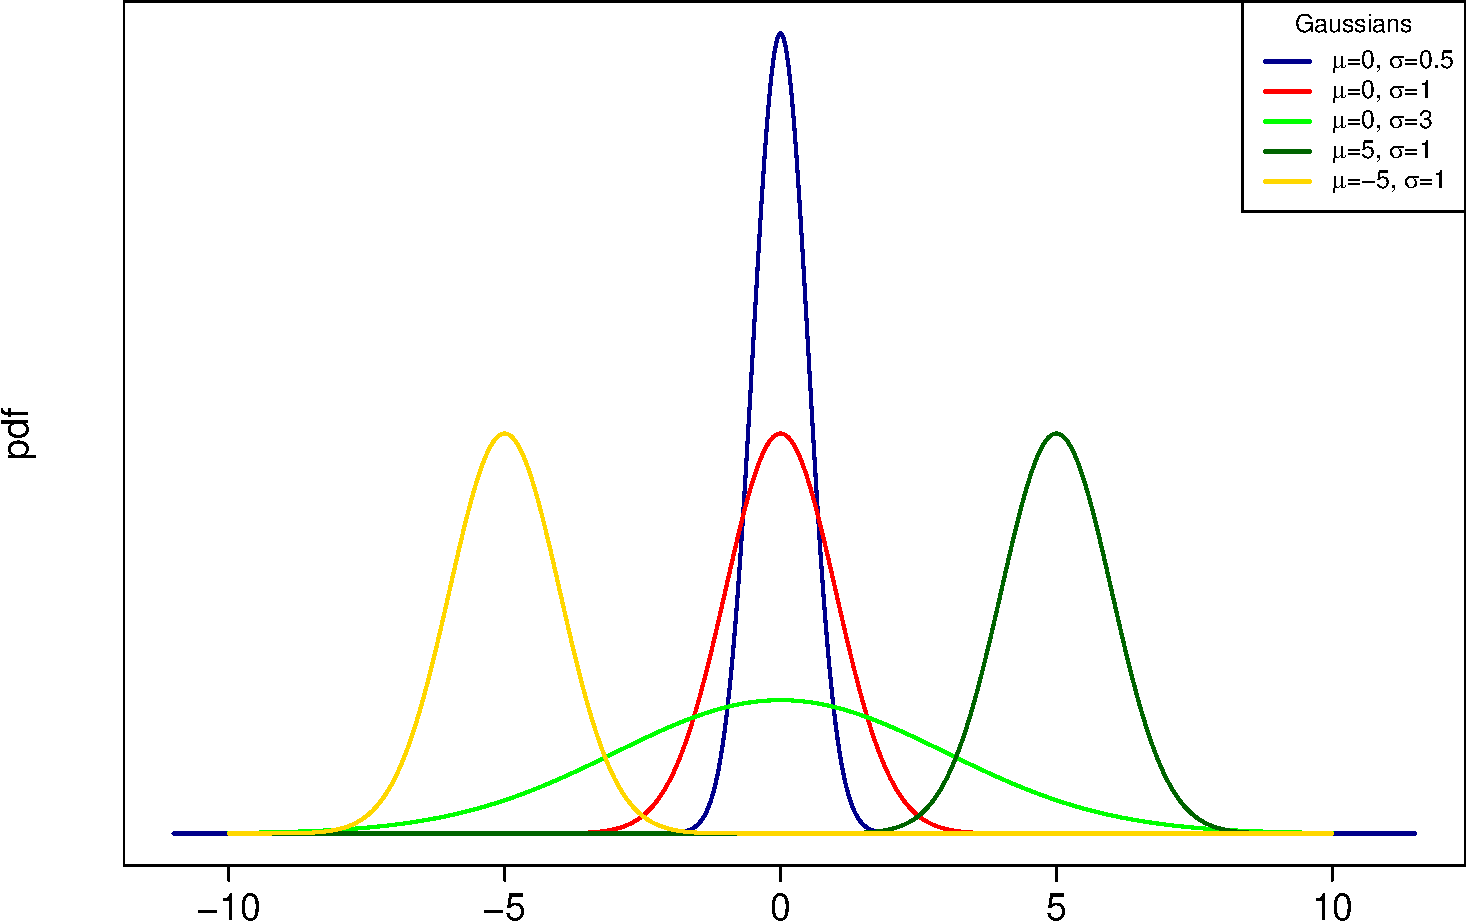
\includegraphics[width=0.65\linewidth]{lecture4_files/figure-beamer/unnamed-chunk-3-1} \end{center}

\end{frame}

\begin{frame}{Joint distribution}
\protect\hypertarget{joint-distribution}{}

Ramdom variable \(\vv{X} = [X_1, X_2, \ldots, X_n]^T\) can be
multidimensional (each \(X_i\) is r.v.)

\begin{itemize}
\tightlist
\item
  essentially a \emph{random vector}
\end{itemize}

\bigskip  Still satisfies the same requirements
\[\forall \vv{x}, 0<P(\vv{X}=\vv{x}) <1,\; \sum_{x_1}\sum_{x_2}\ldots\sum_{x_n} P(\vv{X} =[x_1, x_2, \ldots, x_n]) =1\]

\begin{itemize}
\tightlist
\item
  means the probability that \({X} =\vv{x}\) is jointly true
\end{itemize}

\bigskip

For bivariate case, i.e. \(n=2\), \(X_1, X_2\) are \textbf{independent}
(e.g.~rolling two dice independently) if

\[P(\vv{X}) = P(X_1)P(X_2)\]

\end{frame}

\begin{frame}{Example: joint distribution}
\protect\hypertarget{example-joint-distribution}{}

The joint distribution of \(X\) snow or not, \(Y\in\) \{\text{spring},
\text{summer}, \text{autumn}, \text{winter}\} represents the season that
\(x\) belongs to : \bigskip 

\begin{table}\centering
\begin{tabular}{ l | c | c | c | c}
   \centering                    
   & $y=\text{Spring}$ & $y=\text{Summer}$ &$y=\text{Autumn}$ & $y=\text{winter}$\\ 
   \hline
  $x= F$ & 0.05 & 0.25 & 0.075& 0\\
    \hline 
  $x= T$ & 0.2 & 0 & 0.175& 0.25\\ 
\end{tabular}
\end{table}
\bigskip

It is easy to verify that\\
\[\sum_x\sum_y p(x, y) = 1\]

\end{frame}

\begin{frame}{Probability rules}
\protect\hypertarget{probability-rules}{}

There are only two probability rules (integration for continuous r.v.):

\begin{enumerate}
    \item product rule: \[ p(x, y) = p (y|x)p(x) = p(x|y)p(y)\]
    \item sum rule (marginalisation): \[ p (x) = \sum_y p(x, y),\; p(y) = \sum_x p(x, y)\]
\end{enumerate}

\end{frame}

\begin{frame}{Conditional probability}
\protect\hypertarget{conditional-probability}{}

Conditional probability distribution (by product rule):
\[p (x| y) = \frac{p(x, y)}{p(y)}\]

\begin{itemize}
\tightlist
\item
  probability distribution of \(x\) conditional on the value of \(y\)
\end{itemize}

\bigskip

\begin{table}\centering
\begin{tabular}{ l | c | c | c | c}
   \centering                    
   & $y=\text{Spring}$ & $y=\text{Summer}$ &$y=\text{Autumn}$ & $y=\text{winter}$\\ 
   \hline
  $x= F$ & 0.05 & 0.25 & 0.075& 0\\
    \hline 
  $x= T$ & 0.2 & 0 & 0.175& 0.25\\ 
\end{tabular}
\end{table}

\bigskip

\begin{itemize}
\item
  \(P(Y= \text{Spring})\) ? use sum rule
  \[P(Y = \text{Spring}) = \sum_{x=\{T,F\}} P(X=x,Y=\text{Spring}) =0.05+0.2=\frac{1}{4}\]
\item
  \(P(X=T | Y= \text{Spring})\) ?
  \(P(X=T | y = \text{Spring}) = \frac{P(x=T, y=\text{Spring})}{P(y=\text{Spring})}=\frac{0.2}{0.25}=0.8\)
\end{itemize}

\end{frame}

\begin{frame}{Parameter estimation problem}
\protect\hypertarget{parameter-estimation-problem}{}

Given dataset
\(\mathcal{D} =\{\di{y}{1}, \di{y}{2},\ldots,\di{y}{m}\}\), and assume
\[\di{y}{i} {\sim}  P(\di{y}{i}| \theta), \;  i=1,\ldots, m\]

\begin{itemize}
\tightlist
\item
  \emph{parameter estimation}: given \(\mathcal{D}\), what is
  \(\theta\)?
\end{itemize}

\bigskip

For example, throw the same coin \(n\) times and record value
\(\di{y}{i}\in \{1,0\}, i=1,\ldots,m\)
\[P(\di{y}{i}|\theta) = Ber(\theta)\]

\begin{itemize}
\tightlist
\item
  \(\di{y}{i} \stackrel{iid}{\sim} Ber(\theta)\): independent and
  identically distributed
\item
  \(\theta\): the probability that head turns up
\end{itemize}

\end{frame}

\begin{frame}{Maximum Likelihood Estimation}
\protect\hypertarget{maximum-likelihood-estimation}{}

Likelihood function:
\(P(\mathcal{D}|\theta)= \prod_i^m p(\di{y}{i}|\theta)\)

\begin{itemize}
\tightlist
\item
  the probability of observing data \(\mathcal{D}\) given \(\theta\)
\item
  it is not a probability distribution for \(\theta\):
  \(\int p(\mathcal{D}|\theta) d\theta \neq 1\)
\item
  but it is a function of \(\theta\) (given \(\mathcal{D}\))
\end{itemize}

\bigskip

Maximum likelihood estimation:

\[\theta_{ML} = \argmax_{\theta} P(\mathcal{D}|\theta)\]

\begin{itemize}
\tightlist
\item
  the value \(\theta\) most likely to have generated the data
\end{itemize}

\bigskip

We usually deal with log-likelihood, denoted as \(\mathcal{L}(\theta)\)

\[\theta_{ML} = \argmax_{\theta} \underbrace{\log P(\mathcal{D}|\theta)}_{\mathcal{L}(\theta)}= \argmax_{\theta} P(\mathcal{D}|\theta)\]

\end{frame}

\begin{frame}{MLE for Bernoulli}
\protect\hypertarget{mle-for-bernoulli}{}

For the Bernoulli case: \(\di{y}{i} \in \{1,0\}\) \begin{align}
  \mathcal{L}(\theta) &= \log P(\mathcal{D}|\theta) = \log \prod_{i=1}^m P(\di{y}{i}; \theta)\nonumber \\
  &=  \log \prod_{i=1}^m \theta^{\di{y}{i}}(1-\theta)^{1-\di{y}{i}} \label{eq:berlik}\\
  &= \log (\theta^{\sum_{i=1}^m \di{y}{i}}(1-\theta)^{\sum_{i=1}^m (1-\di{y}{i})}) \nonumber\\
  &= \sum_{i=1}^m \di{y}{i} \log\theta + (m- \sum_{i=1}^m \di{y}{i}) \log (1-\theta) \nonumber\\
  &= R \log\theta + (m- R) \log (1-\theta) \nonumber
  \end{align}

\begin{itemize}
\tightlist
\item
  \(R=\sum_i^m \di{y}{i}\): the total count of heads
\item
  we will use the likelihood function eq.(\ref{eq:berlik}) for logistic
  regression later
\end{itemize}

\end{frame}

\begin{frame}{Some plots of (scaled) likelihood}
\protect\hypertarget{some-plots-of-scaled-likelihood}{}

\begin{columns}
\begin{column}{0.5\textwidth}

\begin{center}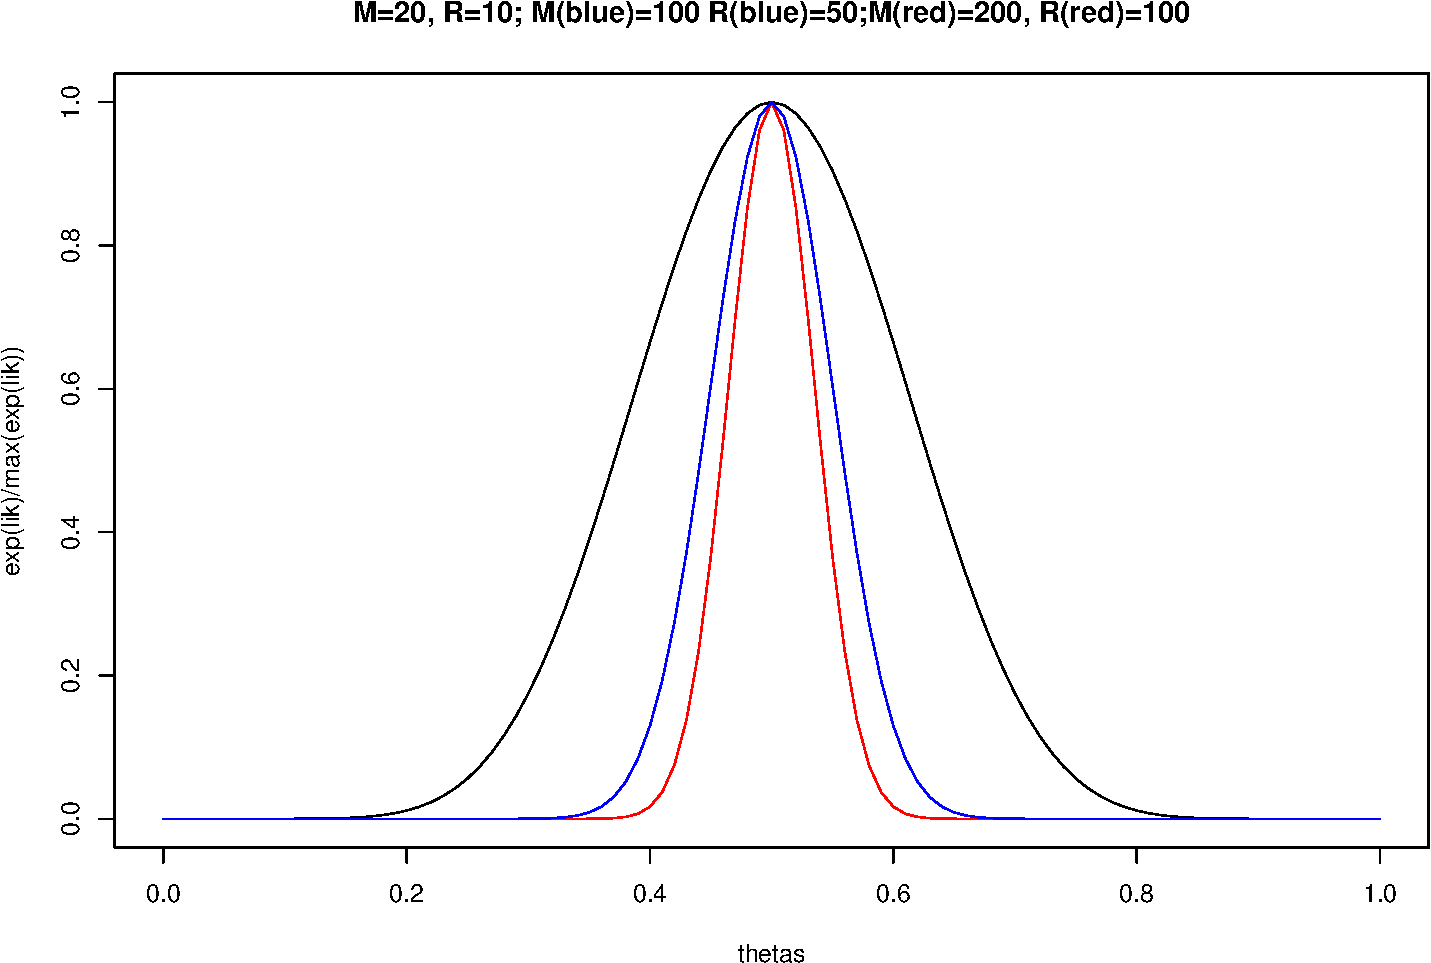
\includegraphics[width=1\linewidth]{lecture4_files/figure-beamer/unnamed-chunk-5-1} \end{center}


 $m=20; R=\sum x_i=10$
 \textcolor{blue}{$m=100; R=\sum{x_i}=50$}
 \textcolor{red}{$m=200; R=\sum{x_i}=100$}
  
  
\end{column}
\begin{column}{0.5\textwidth}

\begin{center}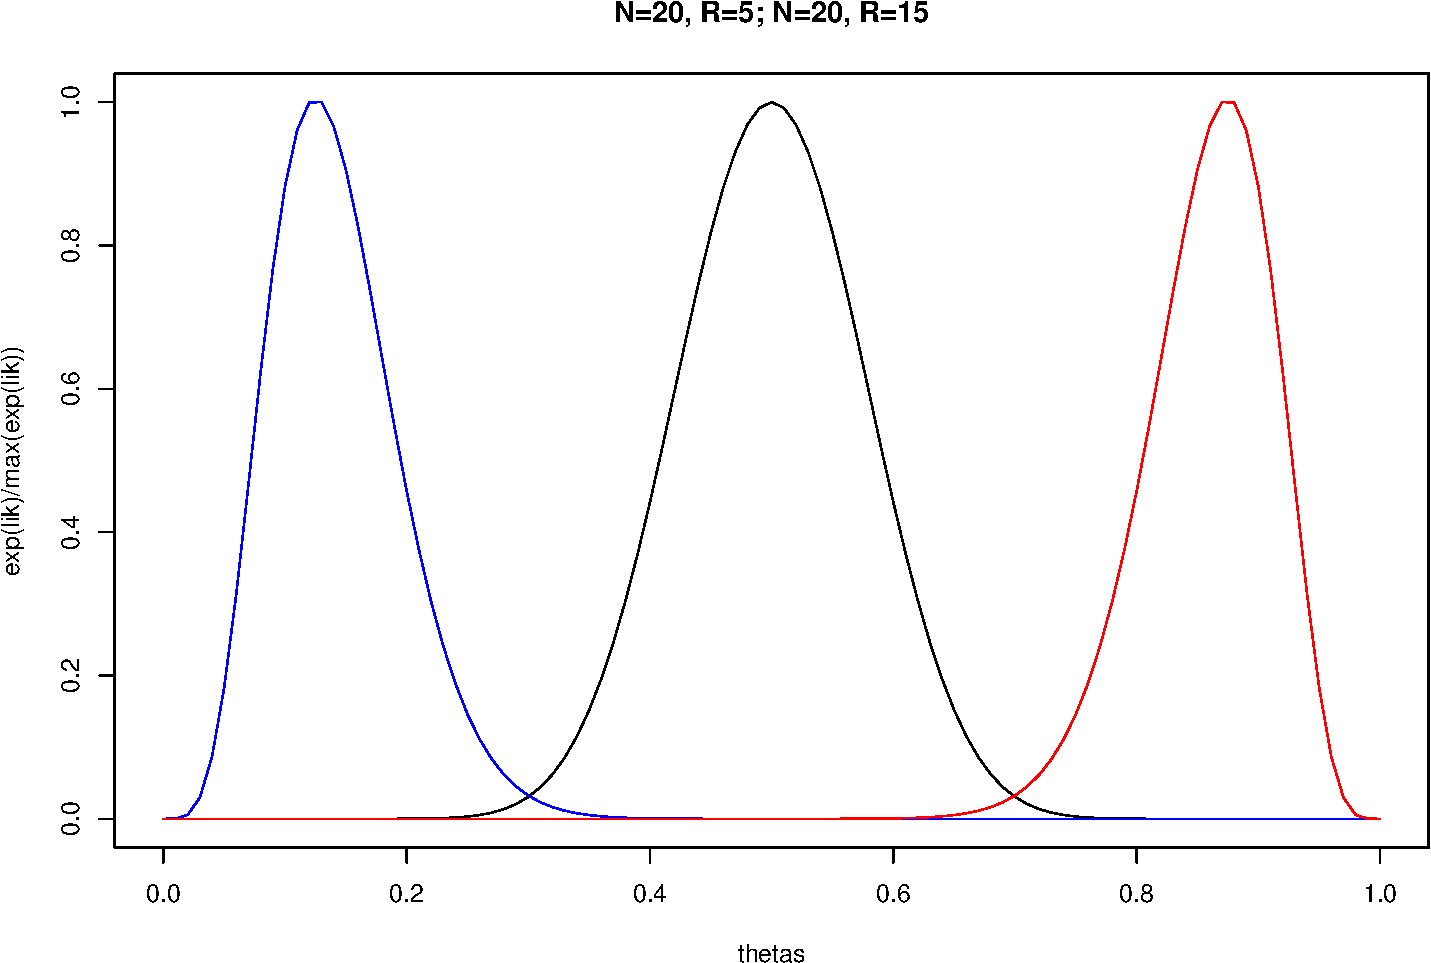
\includegraphics[width=1\linewidth]{lecture4_files/figure-beamer/unnamed-chunk-6-1} \end{center}
 $m=40; R=\sum x_i=20$
 \textcolor{blue}{$m=40; R=\sum{x_i}=5$}
 \textcolor{red}{$m=40; R=\sum{x_i}=35$}
\end{column}

\end{columns}

\end{frame}

\begin{frame}{MLE for Bernoulli}
\protect\hypertarget{mle-for-bernoulli-1}{}

Take the derivative \(\frac{d\mathcal{L}(\theta)}{d\theta}\) and set it
to zero

\begin{align*}
\mathcal{L}(\theta)&= R \log\theta + (m- R) \log (1-\theta) \\
\frac{dL}{d\theta} &= \frac{R}{\theta} - \frac{m-R}{1-\theta} =0 \\
&\Rightarrow \theta_{ML}= \frac{R}{m}
\end{align*}

\begin{itemize}
\tightlist
\item
  note \(R=\sum_{i=1}^m \di{y}{i}\) is the count of heads;
\item
  \(m\) is the total count
\item
  \(\theta_{ML}\) is just the relative frequency
\end{itemize}

\end{frame}

\begin{frame}{Gradient ascent (descent) ?}
\protect\hypertarget{gradient-ascent-descent}{}

We can also apply gradient \textbf{ascent} (why ascent?):

loop until converge:
\[\theta_{t+1} \leftarrow \theta_{t} + \alpha \nabla_{\theta}\mathcal{L}(\theta_t)\]

\begin{itemize}
\tightlist
\item
  where
  \[\nabla_{\theta} \mathcal{L}(\theta) = \frac{R}{\theta} - \frac{m-R}{1-\theta}\]
\end{itemize}

or gradient descent with negative log likelihood
\(N\mathcal{L}(\theta)=-\mathcal{L}(\theta)\):
\[\theta_{t+1} \leftarrow \theta_{t} - \alpha \nabla_{\theta}(N\mathcal{L}(\theta_t))\]

\begin{itemize}
\tightlist
\item
  but \(\theta \in [0,1]\): constrained optimisation
\item
  the gradient \(\nabla_{\theta} \mathcal{L}(\theta)\) is not defined at
  \(\theta = 0, 1\) !\\
\item
  difficult to converge if step outside:
  \(\theta_t \geq 1; \theta_t\leq 0\)
\end{itemize}

\end{frame}

\begin{frame}{Reparameterisation trick for gradient descent (ascent)}
\protect\hypertarget{reparameterisation-trick-for-gradient-descent-ascent}{}

Reparameterisation trick: find \(f\)
\[\theta = f(\beta), \; \text{such that}\]

\begin{itemize}
\tightlist
\item
  \(\beta \in R\) and write
  \(\mathcal{L}(\theta) = \mathcal{L}(f(\beta))\)
\item
  use chain rule to find
  \(\nabla_{\beta}\mathcal{L}(\beta) = \nabla_{\theta}\mathcal{L}\cdot\nabla_{\beta}f(\beta)\)
\item
  gradient ascent against \(\beta\); then transform back
\end{itemize}

\[
  \beta_{t+1} \leftarrow \beta_{t} + \alpha \nabla_{\beta}\mathcal{L}(\beta_t);\;\; \theta_{t+1} \leftarrow f(\beta_{t+1}) 
\]

\bigskip

For example, if \(\theta > 0\), then
\[\theta = f(\beta) = e^{\beta}, \text{ the new gradient is then}\]

\[\nabla_{\beta}\mathcal{L}(\beta) = \nabla_{\theta}\mathcal{L}\cdot e^{\beta}\]

\end{frame}

\begin{frame}{Reparameterisation trick for Bernoulli MLE}
\protect\hypertarget{reparameterisation-trick-for-bernoulli-mle}{}

For \(\theta \in [0,1]\), such a function is sigmoid:

\begin{columns}
\begin{column}{0.4\textwidth}
$$\sigma(x) = \frac{1}{1+e^{-x}} = \frac{e^x}{e^x+1};$$
The derivative: 
$$\frac{d\sigma(x)}{dx} = \sigma(x)(1-\sigma(x))$$
\end{column}

\begin{column}{0.6\textwidth}

\begin{center}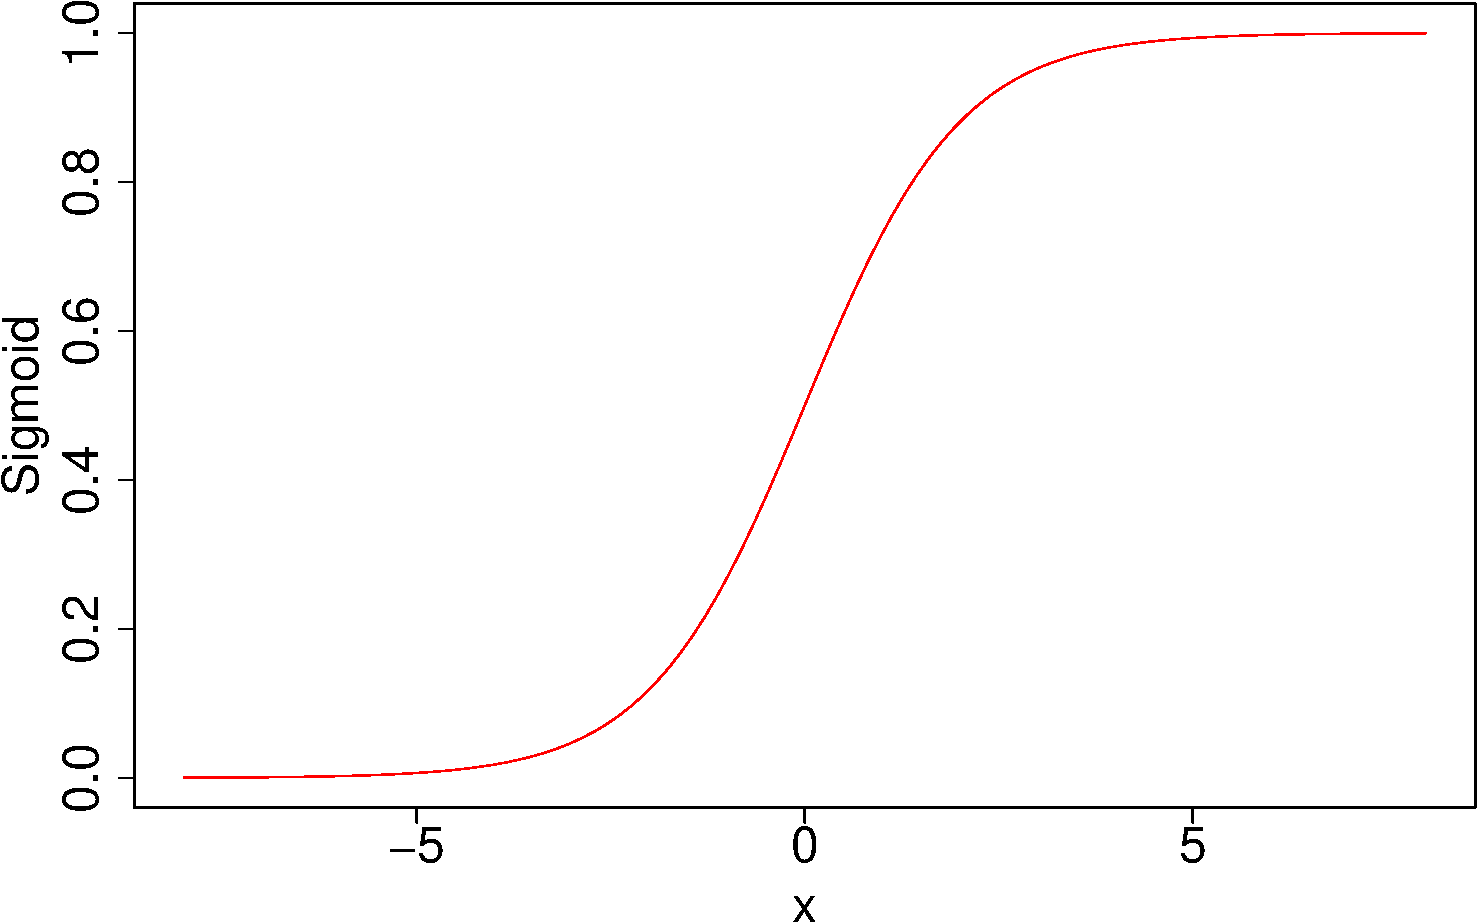
\includegraphics[width=1\linewidth]{lecture4_files/figure-beamer/unnamed-chunk-7-1} \end{center}
\end{column}
\end{columns}

\end{frame}

\begin{frame}{Reparameterisation trick for Bernoulli MLE}
\protect\hypertarget{reparameterisation-trick-for-bernoulli-mle-1}{}

For the Bernoulli case, reparameterize \(\theta\):
\[\theta = \sigma(\beta);\]

Rewrite the log likelihood \(\mathcal{L}\) as a function of \(\beta\):

\[\mathcal{L}(\beta) = \log \prod_{i=1}^m \theta^{\di{y}{i}}(1-\theta)^{1-\di{y}{i}}= \log \prod_{i=1}^m \sigma(\beta)^{\di{y}{i}}(1-\sigma(\beta))^{1-\di{y}{i}}\]
The gradient of \(L\) w.r.t \(\beta\) is

\[\nabla_\beta \mathcal{L}(\beta) = \nabla_{\theta} \mathcal{L} \cdot \nabla_\beta{\theta} = \left(\frac{R}{\sigma} - \frac{m-R}{1-\sigma}\right)\sigma(1-\sigma)\]

\end{frame}

\begin{frame}[fragile]{Code (R like syntax)}
\protect\hypertarget{code-r-like-syntax}{}

\begin{Shaded}
\begin{Highlighting}[]
\NormalTok{grad <-}\StringTok{ }\ControlFlowTok{function}\NormalTok{(m,r,beta)\{}
\NormalTok{  sig <-}\StringTok{ }\KeywordTok{sigmoid}\NormalTok{(beta)}
\NormalTok{  g <-}\StringTok{ }\NormalTok{(r}\OperatorTok{/}\NormalTok{sig }\OperatorTok{-}\StringTok{ }\NormalTok{(m}\OperatorTok{-}\NormalTok{r)}\OperatorTok{/}\NormalTok{(}\DecValTok{1}\OperatorTok{-}\NormalTok{sig))}\OperatorTok{*}\NormalTok{sig}\OperatorTok{*}\NormalTok{(}\DecValTok{1}\OperatorTok{-}\NormalTok{sig)}
  \KeywordTok{return}\NormalTok{(g)}
\NormalTok{\}}

\NormalTok{berGAscent <-}\StringTok{ }\ControlFlowTok{function}\NormalTok{(alpha, iter, m, r, beta0)\{}
\NormalTok{  betas <-}\StringTok{ }\KeywordTok{vector}\NormalTok{(}\DataTypeTok{mode=}\StringTok{"numeric"}\NormalTok{, }\DataTypeTok{length =}\NormalTok{ iter}\OperatorTok{+}\DecValTok{1}\NormalTok{)}
\NormalTok{  betas[}\DecValTok{1}\NormalTok{] <-}\StringTok{ }\NormalTok{beta <-}\StringTok{ }\NormalTok{beta0}
  \ControlFlowTok{for}\NormalTok{(i }\ControlFlowTok{in} \DecValTok{1}\OperatorTok{:}\NormalTok{iter)\{}
\NormalTok{    g <-}\StringTok{ }\KeywordTok{grad}\NormalTok{(m,r,beta)}
\NormalTok{    betas[i}\OperatorTok{+}\DecValTok{1}\NormalTok{] <-}\StringTok{ }\NormalTok{beta <-}\StringTok{ }\NormalTok{beta }\OperatorTok{+}\StringTok{ }\NormalTok{alpha}\OperatorTok{*}\NormalTok{g}
\NormalTok{  \}}
  \KeywordTok{return}\NormalTok{(betas)}
\NormalTok{\}}
\end{Highlighting}
\end{Shaded}

\end{frame}

\begin{frame}{Example with
\(m=100, R=25, \theta_{ML} = 0.25, \alpha=0.01\)}
\protect\hypertarget{example-with-m100-r25-theta_ml-0.25-alpha0.01}{}

\begin{center}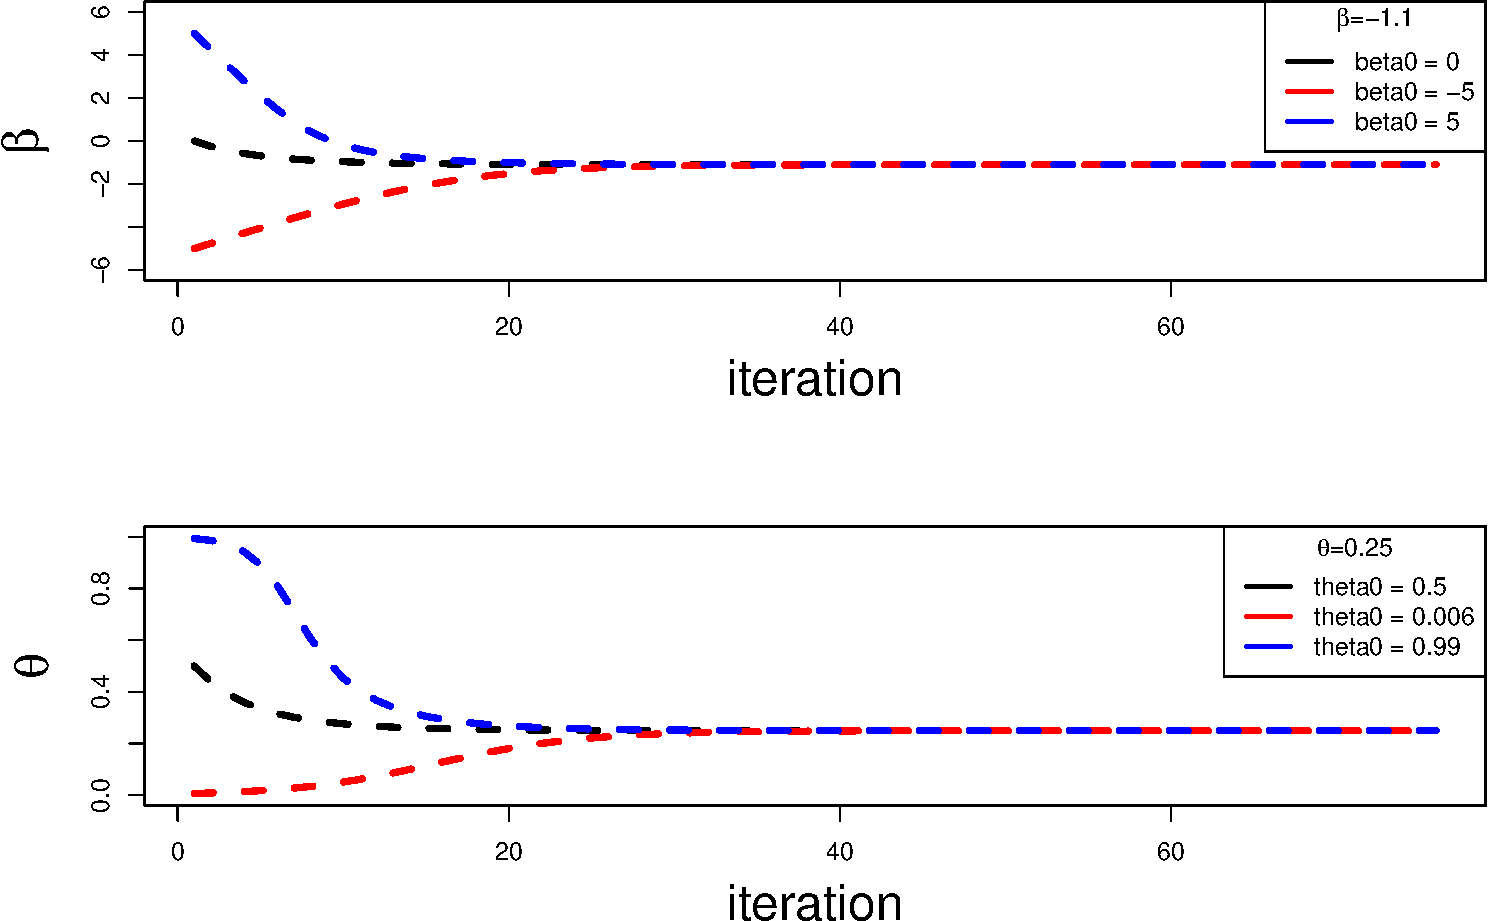
\includegraphics[width=1\linewidth]{lecture4_files/figure-beamer/unnamed-chunk-9-1} \end{center}

\end{frame}

\begin{frame}{MLE for Gaussian}
\protect\hypertarget{mle-for-gaussian}{}

Similarly, for Gaussian
\(\mathcal{D}=\{\di{y}{1}, \ldots, \di{y}{m}\}\), the parameters are
\(\vv{\theta} = \{\mu, \sigma^2\}\) and

\[p(\di{y}{i}; \mu, \sigma^2) = \Gaussian{\di{y}{i}}{\mu}{\sigma}\]

therefore, the log likelihood for \(\di{y}{i}\) is:
\[\log p(\di{y}{i}; \mu, \sigma^2) = -\frac{1}{2} \log(2\pi\sigma^2) -\frac{1}{2\sigma^2}\underbrace{(\di{y}{i}-\mu)^2}_{\text{squared error!}}\]

\end{frame}

\begin{frame}{}
\protect\hypertarget{section}{}

\begin{align}
  \mathcal{L}(\mu, \sigma^2) &= \log p(\mathcal{D}|\mu, \sigma^2) = \log \prod_{i=1}^m p(\di{y}{i}; \mu, \sigma^2) = \sum_{i=1}^m \log p(\di{y}{i};\mu, \sigma^2)  \nonumber \\ &= \sum_{i=1}^m \left(-\frac{1}{2} \log(2\pi\sigma^2) -\frac{(\di{y}{i}-\mu)^2}{2\sigma^2}\right ) \nonumber \\
  &= -\frac{m}{2}\log(2\pi \sigma^2)- \frac{1}{2\sigma^2} \underbrace{\sum_{i=1}^m (\di{y}{i}-\mu)^2}_{\text{sum of squared error}} \nonumber
  \end{align}

Take (partial) derivative and set to zero (verify yourself!):
\[\frac{\partial L}{\partial \mu} =  \frac{1}{\sigma^2} \left (\sum_{i=1}^m (\di{y}{i}-\mu)\right) = 0; \;
\frac{\partial L}{\partial \sigma^2} =-\frac{m}{2\sigma^2} +\frac{\sum_{i=1}^m(\di{y}{i} -\mu)^2}{2(\sigma^2)^2}  = 0\]

\begin{align*} 
\Rightarrow \begin{cases} \mu_{ML} = \frac{1}{m}\sum_{i=1}^m \di{y}{i} \;\; \leftarrow \text{ sample mean!} \\
\sigma^2_{ML} = \frac{1}{m}\sum_{i=1}^m(\di{y}{i}-\mu_{ML})^2
\end{cases}
\end{align*}

\end{frame}

\begin{frame}{Linear regression: revisit}
\protect\hypertarget{linear-regression-revisit}{}

Linear regression model:
\[y^{(i)} =\vv{\theta}^T\vv{x}^{(i)}  + e^{(i)}\]

\begin{itemize}
\tightlist
\item
  \(i = 1,\ldots,m\): index of data samples (row index),
\item
  \(\vv{x}^{(i)} = [1, x_{1}^{(i)}, \ldots, x^{(i)}_n]^T\) is a
  \((n+1) \times 1\) vector:

  \begin{itemize}
  \tightlist
  \item
    \(n\): number of predictors (columns)
  \end{itemize}
\item
  \(\vv{\theta}\) is the model parameter
\item
  \(e^{(i)}\) is the prediction difference
\end{itemize}

Assume \[\di{e}{i} \sim \normal{0}{\sigma^2}\]

\begin{itemize}
\tightlist
\item
  the prediction error is Gaussian distributed
\item
  the mean of the error is \(0\)
\item
  the variance is \(\sigma^2\), which needs to be estimated
\end{itemize}

\end{frame}

\begin{frame}{Linear regression: revisit}
\protect\hypertarget{linear-regression-revisit-1}{}

\[\di{e}{i}  \sim \normal{0}{\sigma^2}\] \[\Downarrow\]

\[\di{y}{i}=\vv{\theta}^{T} \di{\vv{x}}{i} + \di{e}{i}  \sim \normal{\vv{\theta}^{T} \di{\vv{x}}{i}}{\sigma^2}\]

\[\Downarrow\]

\[p(\di{y}{i}|\vv{\theta},\sigma^2, \di{\vv{x}}{i}) = \frac{1}{\sqrt{2\pi\sigma^2}}\text{exp}\left(-\frac{(\di{y}{i}-\vv{\theta}^T\di{\vv{x}}{i})^2}{2\sigma^2}\right)\]
\[\Downarrow\]

\[\mathcal{L}(\vv{\theta},\sigma^2) = \log p(\mathcal{D} |\vv{\theta}, \sigma^2) = \log p(\vv{y} |\vv{\theta},\sigma^2,\vv{X})= \log \prod_{i=1}^m p(\di{y}{i};\vv{\theta},\di{\vv{x}}{i})\]

\end{frame}

\begin{frame}{Linear regression: maximum likelihood estimation}
\protect\hypertarget{linear-regression-maximum-likelihood-estimation}{}

The log likelihood function is: \begin{align*}
\mathcal{L}(\vv{\theta}, \sigma^2) &= \log \prod_{i=1}^m p(\di{y}{i};\vv{\theta},\di{\vv{x}}{i}) \\
&= \sum_{i=1}^m \log p(\di{y}{i};\vv{\theta},\di{\vv{x}}{i}) \\
&= -\frac{m}{2}\log(2\pi\sigma^2) - \frac{1}{2\sigma^2}\sum_{i=1}^m (\di{y}{i} - \vv{\theta}^T\di{\vv{x}}{i})^2
\end{align*}

\bigskip

Maximising \(\mathcal{L}\) w.r.t \(\vv{\theta}\) is the same as
minimising loss function
\[L(\vv{\theta})=\sum_{i=1}^m (\di{y}{i} - \vv{\theta}^T\di{\vv{x}}{i})^2\]

\[\Rightarrow \vv{\theta}_{ML} = \vv{\theta}_{LS}\]

\end{frame}

\begin{frame}{Logistic regression}
\protect\hypertarget{logistic-regression}{}

Let's consider binary classification \(\di{y}{i} \in \{1,0\}\), assume
Bernoulli likelihood

\[P(y^{(i)}=1) = \sigma\left (\vv{\theta}^T\vv{x}^{(i)}\right )\]

\begin{itemize}
\tightlist
\item
  \(i = 1,\ldots,m\): index of data samples (row index)
\item
  \(\vv{\theta}^T\di{\vv{x}}{i}= \theta_0 + \theta_1\di{x_1}{i}+\ldots+ \theta_n\di{x_n}{i}\in R\)
\item
  \(\sigma(x) \in [0,1]\)
\item
  \(\vv{\theta}\) is the model parameter
\end{itemize}

The log likelihood function is

\[\mathcal{L}(\vv{\theta}) = \underbrace{\log \prod_{i=1}^m \sigma^{\di{y}{i}} (1-\sigma)^{1-\di{y}{i}}}_{\text{the same as Bernoulli model with } \theta}\]

\begin{itemize}
\tightlist
\item
  replace single parameter \(\sigma(\beta)\) with
  \(\sigma(\vv{\theta}^T\di{\vv{x}}{i})\)
\item
  \(\beta\) serves the same purpose as \(\theta_0\): the intercept
  (cf.~page 22)
\end{itemize}

\end{frame}

\begin{frame}{Logistic regression: geometric view}
\protect\hypertarget{logistic-regression-geometric-view}{}

\[\sigma(\vv{\theta}^T\vv{x})\]

\begin{itemize}
\tightlist
\item
  \(\vv{\theta}^T\vv{x}\) is a hyperplane
\item
  \(\sigma(\vv{\theta}^T\vv{x})\) squeeze the plane between \((0, 1)\)
\item
  \(\vv{\theta}\) determines the direction of surface facing
\item
  \(||\vv{\theta}||_2^2\) determines the steepness
\end{itemize}

\end{frame}

\begin{frame}{}
\protect\hypertarget{section-1}{}

\begin{figure}
    \centering
    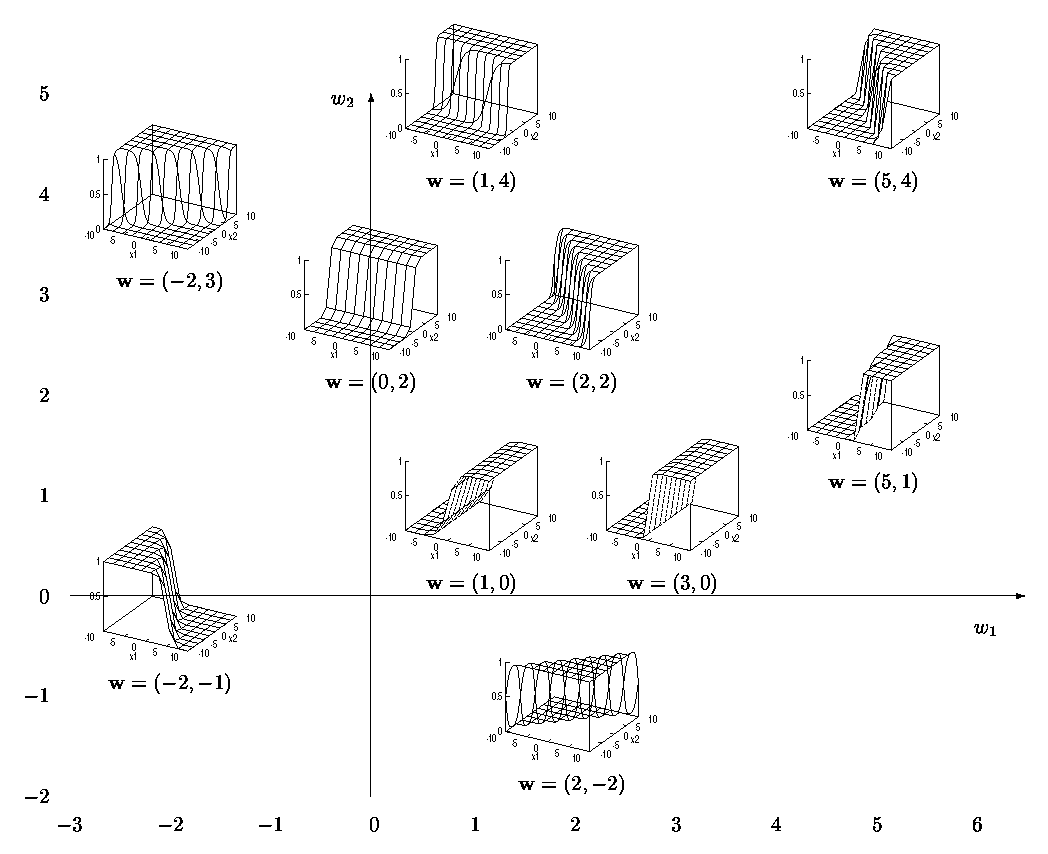
\includegraphics[width = 0.85\textwidth]{./figs/figure260.eps}\footnote{Information theory, inference and learning algorithms, David MacKay}
 % \caption{Awesome figure}
\end{figure}

\end{frame}

\begin{frame}{Summary}
\protect\hypertarget{summary}{}

Maximum likelihood estimation

\begin{itemize}
\tightlist
\item
  gives rise to squared error loss function for regression

  \begin{itemize}
  \tightlist
  \item
    sample mean is the simplest kind of linear regression where
    \(x^{(i)}=1\) for all \(i=1,\ldots,m\)
  \end{itemize}
\item
  gives rise to logistic error (cross-entropy) for classification

  \begin{itemize}
  \tightlist
  \item
    relative frequency is the simpliest kind of logistic regression
    where \(x^{(i)}=1\) for all \(i=1,\ldots,m\)
  \end{itemize}
\end{itemize}

\end{frame}

\begin{frame}{Suggested reading and exercises}
\protect\hypertarget{suggested-reading-and-exercises}{}

Reading

\begin{itemize}
\tightlist
\item
  MLAPP 2.2, 2.3.1, 2.3.2, 2.4.1, 7.3, 8.1-8.3.1
\item
  DL 3, 5.5, 5.7.1
\item
  Information theory, inference and learning algorithms by David MacKay,
  chapter 2, 22.1, 39.1, 39.2
\end{itemize}

\bigskip

Exercise

\begin{itemize}
\tightlist
\item
  go through the equations
\item
  write gradient descent for Gaussian model's likelihood function

  \begin{itemize}
  \tightlist
  \item
    generate some artifical data
  \item
    workout the gradients
  \item
    use the reparameterisation trick to treat \(\sigma^2 >0\)
  \item
    check whether they converge
  \end{itemize}
\item
  derive the gradient for logistic regression's log likelihood function
\end{itemize}

\end{frame}

\begin{frame}{Next time}
\protect\hypertarget{next-time}{}

\begin{itemize}
\item
  Large number theory of MLE

  \[\theta_{ML} \rightarrow \mathcal{N}(\theta, I_m^{-1}(\theta))\]

  \begin{itemize}
  \tightlist
  \item
    ML estimator can recover the true parameter \(\theta\)
  \item
    as data size \({m\rightarrow \infty}\)
  \end{itemize}
\item
  gradient descent of logistic regression
\item
  Newton's method for optimisation
\end{itemize}

\end{frame}

\begin{frame}{*Random variable: formal aspects}
\protect\hypertarget{random-variable-formal-aspects}{}

Formally, r.v. \(X\) is a mapping from \emph{sample space} \(\Omega\) to
\emph{target space} \(\mathcal{T}\)

\begin{itemize}
\tightlist
\item
  \(\Omega\): all possible outcomes of an experiment
\item
  \(\mathcal{T}\): possible values \(X\) can take
\item
  events \(E\subseteq \Omega\)
\item
  \(X(\omega) \in \mathcal{T}, \forall \omega \in \Omega\)
\item
  \(X^{-1}\) defines a partition of \(\Omega\) 
\end{itemize}

Example: toss a fair coin twice, r.v. \(X\): \# of heads turned up

\begin{itemize}
\tightlist
\item
  the \emph{sample space} is \(\Omega =\{HH, TT, HT, TH\}\)
\item
  \emph{target space} is \(T =\{0,1,2\}\)
\item
  \(X(HH) = 2; X(HT)=X(TH)=1; X(TT) =0\)
\item
  \(X^{-1} = \{E_0, E_1, E_2\}\) defines a parition of \(\Omega\):
  \(E_0=\{TT\}, E_1=\{TH,HT\}, E_2=\{HH\}\)

  \begin{itemize}
  \tightlist
  \item
    disjoint: \(E_0 \cap E_1 = E_0 \cap E_2= E_1 \cap E_2 = \emptyset\)
  \item
    complete: \(E_0 \cup E_1 \cup E_2 = \Omega\)
  \end{itemize}
\end{itemize}

\end{frame}

\end{document}
